\section[Сучасні можливості]{Сучасні можливості лапароскопічної резекційної хірургії печінки}

\subsection{Анатомічні резекції печінки}
	
З моменту першої \acrshort{llr} можливості методу значно поширились за межі крайових резекцій новоутворень невеликого розміру. На данний момент показана доступність виконання в лапароскопічному варіанті абсолютно всіх видів анатомічних резекцій печінки при доброякісних та онкологічних пухлинах, включно навіть з операціями при хіларній холангіокарциномі. Найбільш часто вживані резекції, такі як \acrshort{llls}, лівобічна та правобічна гемігепатектомія та моносегментектомії є добре вивченими та стандартизованими процедурами, що дозволяє деяким спеціалізованим центрам \cite{Garbarino2019} виконувати до 80-90\% всіх резекцій печінки в лапароскопічному варіанті.

За об'ємом розрізняють малі (Minor) та великі або обширні (Major) резекції. До малих резекцій відносять моно- та бісегментектомії антеролатеральних сегменітв та ліву латеральну секцієектомію. До великих або обширних анатомічних \acrshort{llr} відностяь резекції при яких виляляють три або більше розташованих поруч сегмента. Класичними представниками великих резекцій є лівобічна та правобічна гемігепатектомії, правобічна передня та задня секцієектомії, мезогепатектомія.

\subsubsection{Лівобічна гемігепатектомія}

Лапароскопічна лівобічна гемігепатектомія (\acrshort{llhe}) показала себе як доступна, безпечна та ефективна процедура для пацієнтів, що мають новоутворення лівої долі печінки (Рис. \ref{fig:LeftLobe}). В ретроспективному порівняльному аналізі 62 \acrshort{llhe} та 118 відкритих лівобічних гемігепатектомій у пацієнтів з гепатоцеллюлярною карциномою (\acrshort{hcc}), внутрішньопечінковою холангіокарциномою (\acrshort{ihcc}) та деякими доброякісними новоутвореннями показано перевагу лапароскопічних втручаннь за рахунок зменшення крововтрати, часу до відновлення харчування та частоти важких ускладненнь з порівняними показниками виживаності у онкологічних хворих \cite{Cho2018b}.   

Міжнародне мультицентрове ретроспективне дослідження реузльтатів 82 \acrshort{llhe} \cite{Belli2013a} не виявило достовірної різниці кількості ускладненнь та періопераційних показників у порівнянні з 222 \acrshort{llls}, - процедурою, яка є визнаним "золотим стандартом". Не дивлячись на те, що \acrshort{llhe} є технічно складнішою за \acrshort{llls}, автори рекомендують її в якості стандартного методу лікування. 

\begin{figure}[h]
\caption{Лапароскопічна лівобічна гепмігепатектомія з приводу ехінококозу}

\includegraphics[width=0.9\textwidth]{Illustrations/Chapter_01/LeftLobe_Horizontal.jpg}
\label{fig:LeftLobe}

\medskip
\small
 а), б) - передопераційний та інтраопераційний вигляд ехінококової кисти, в) - диссекція лівих портальних структур. На схемі кольорами помічено: червоний - власна, ліва та права печінкові артерії, синім - горизонтальна порція лівої ворітної вени, зеленим - хіларне плато та лівий жовчний проток, г) - етап транссекції паренхіми, д) - заключний вигляд після резекції, в площині резекції - серединна печінкова вена, зображена синім.

\end{figure}

\subsubsection{Правобічна гемігепатектомія}

Лапароскопічна правобічна гемігепатектомія (\acrshort{lrhe}) є складним втручанням, так як потребує повної мобілізації та маніпуляцій з об'ємною правою долею печінки та вимагає технічної майстерності від оперуючого хірурга (Рис. \ref{fig:RightLobe}). З моменту першого виконання Hüscher C. в 1995 році \cite{Huscher1997} техніка \acrshort{lrhe} вдосконалювалась та зазнавала постійних модифікацій \cite{Gayet2007, Dagher2008, Homma2019, Kim2017a}. В сучасному варіанті \acrshort{lrhe} є добре вивченою процедурою. Її онкологічна еффективність та рівень ускладнень у пацієнтів з ГЦК на фоні цирозу не відрізняється від традиційної відкритої правобічної гемігепатектомії за результатами корейського моноцентрового ретроспективного псевдорандомізованого дослідження \cite{Yoon2017b}. 

\begin{figure}[h]
\caption{Лапароскопічна правобічна гепмігепатектомія}

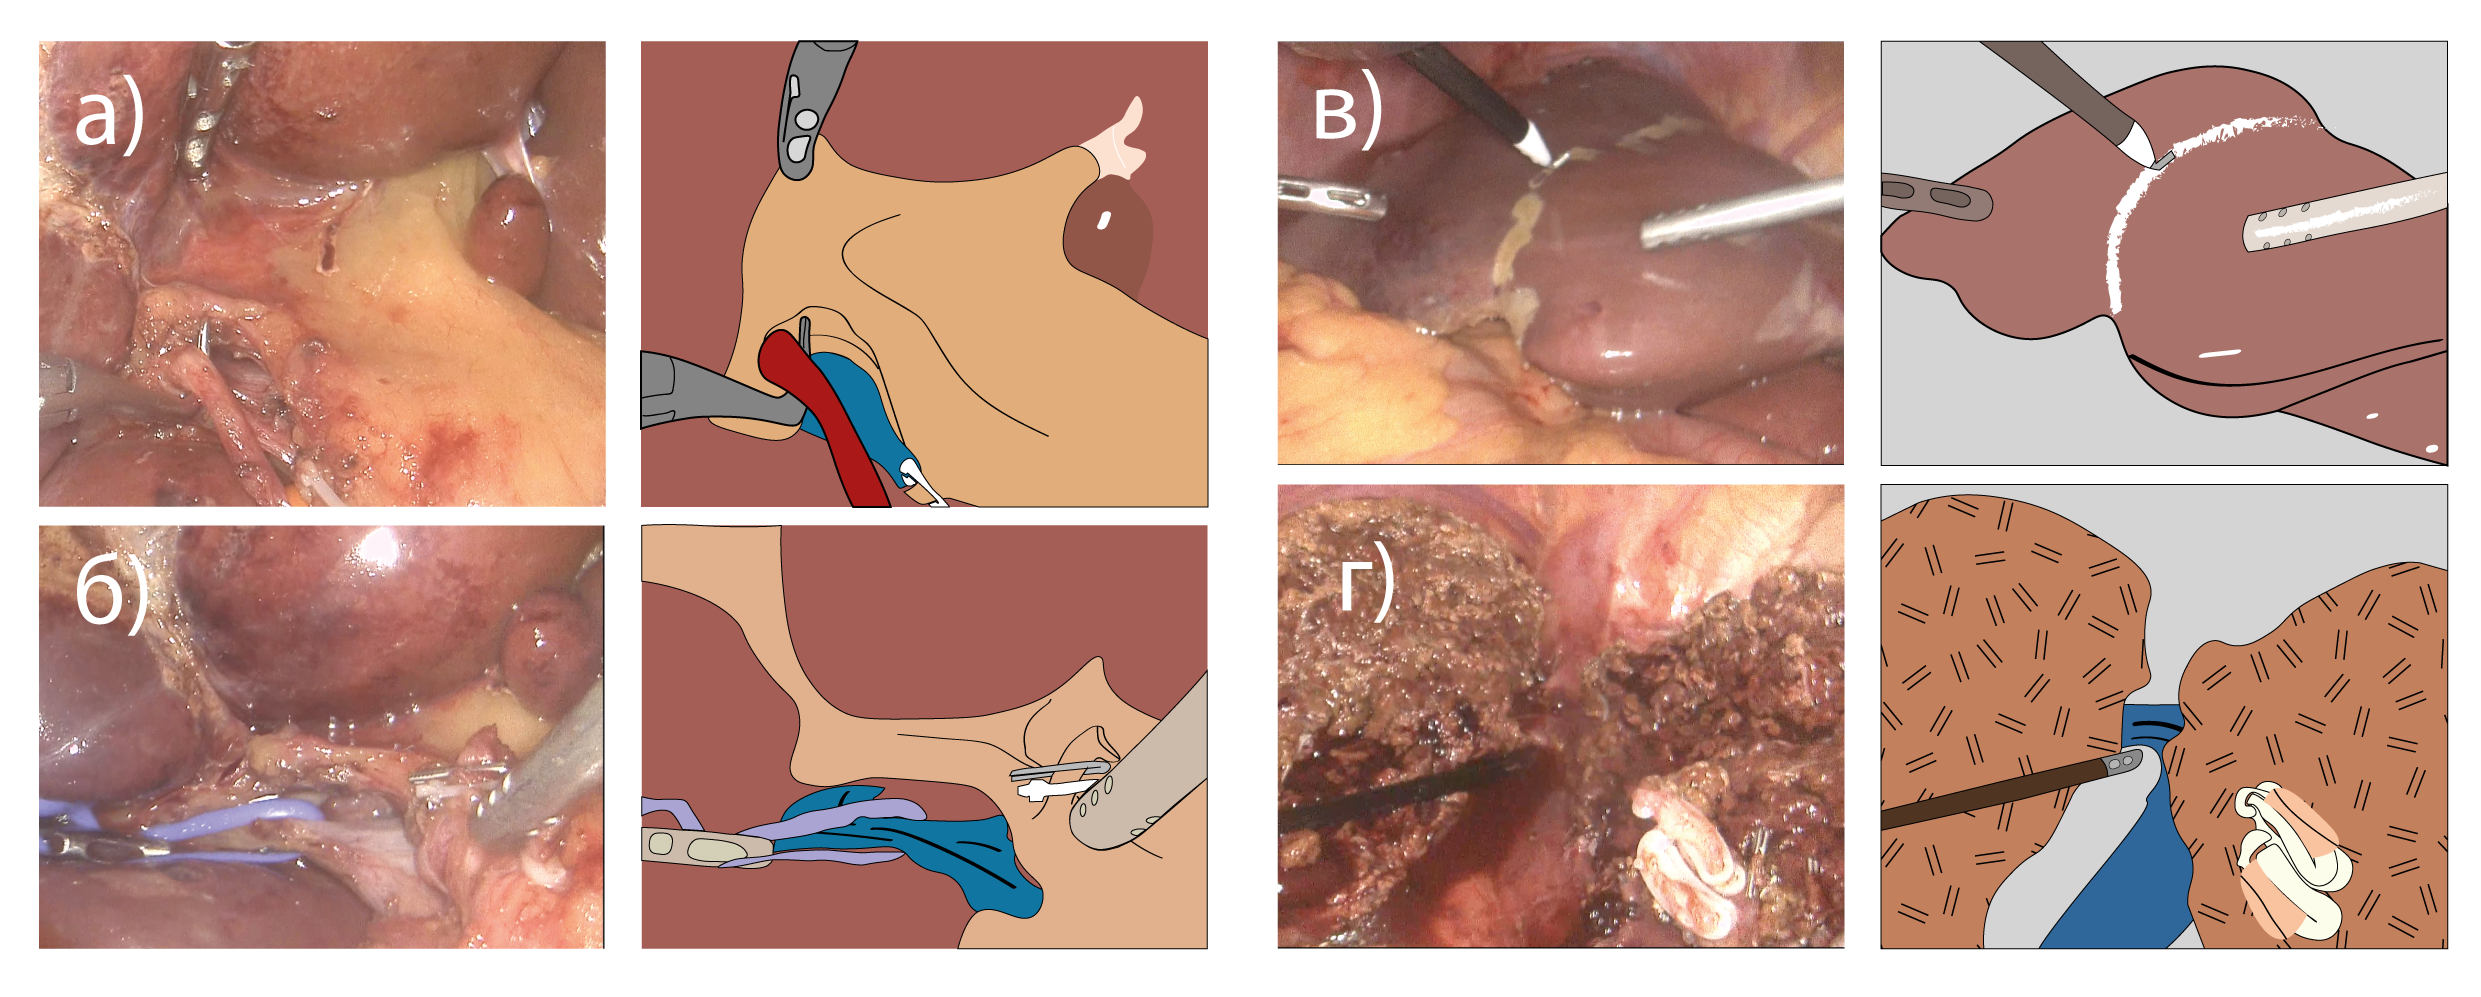
\includegraphics[width=0.9\textwidth]{Illustrations/Chapter_01/RightLobe_Horizontal.png}
\label{fig:RightLobe}

\medskip
\small
а) диссекція правої печінкової артерії, б) диссекція правої ворітної вени, в) намічення лінії транссекції паренхіми вздовж лінії Кантля, г) виконана транссекція паренхіми, виділена права печінова вена.


\end{figure}

\subsubsection{Секцієектомії та центральні резекції}

Окрім \acrshort{llhe} та \acrshort{lrhe} обширні резекції включають в себе праву передню, праву задню та ліву медіальну секцієектомії, мезогепатектомію. Технічно такі операції вважаються складнішими за класичні гемігепатектомії, так як включають дві площини резекції, що знаходяться під кутом одна до одної. Не дивлячись на це, в серії дослідженнь показано, що такі втручання є безпечними та відтворюваними в експертних центрах \cite{Honda2014, Cheng2015, Kim2017, Siddiqi2018}. 

\subsubsection{Складні локалізації}

Постерокраніальні сегменти (Sg 7,8) та каудальна лобектомія певний час вважались недоступними для лапароскопічного доступу через високе незручне розтажування обмежене ребрами та куполом діафрагми, та анатомічну близкість до печінкових вен та нижньої порожнистої вени (\acrshort{ivc}). В 2014 роци Ban D. та співавтори розробили шкалу складності для \acrshort{llr}, де віднесли ізольовані лапароскопічні резекції Sg 7 та 8 до резекцій вищого ступеню складності, порівняно з резекціями інших анатомічних ділянок. Для полегшення доступу до постерокраніальних сегментів Ikeda T. була запропонована напівпронована позиція пацієнта та латеральний доступ до Sg 7-8 \cite{Ikeda2014}.

Пізніше Honda G. та співавторами була опублікована методика анатомичної резекції Sg 7 з внутрішньопечінковим доступом до сегментарного  гліссону \cite{Okuda2017}, а Inoue Y. показано спосіб резекції Sg 6, 7 та 8 з латерального доступу з використанням трансторакальних троакарів \cite{Inoue2017}.  Такж описаний метод виконання атипових резекцій печінки трансторокальним доступом при вираженому злуковому процесі в черевній порожнині \cite{Kruger2014}. Суть методу полягає в доступі до Sg 8 з правої плевральної порожнини шляхом розсічення правого куполу діафрагми.

На теперішній момент анатомічні \acrshort{llr} Sg 7 та 8 печінки є доступними та стандартизованими втручаннями (Рис. \ref{fig:Complex_localisation_Sg7}, \ref{fig:Complex_localisation_Sg8}) 


\begin{figure}[h]
\caption{Лапароскопічна анатомічна резекція Sg 7 з приводу HCC у виконанні авторів}

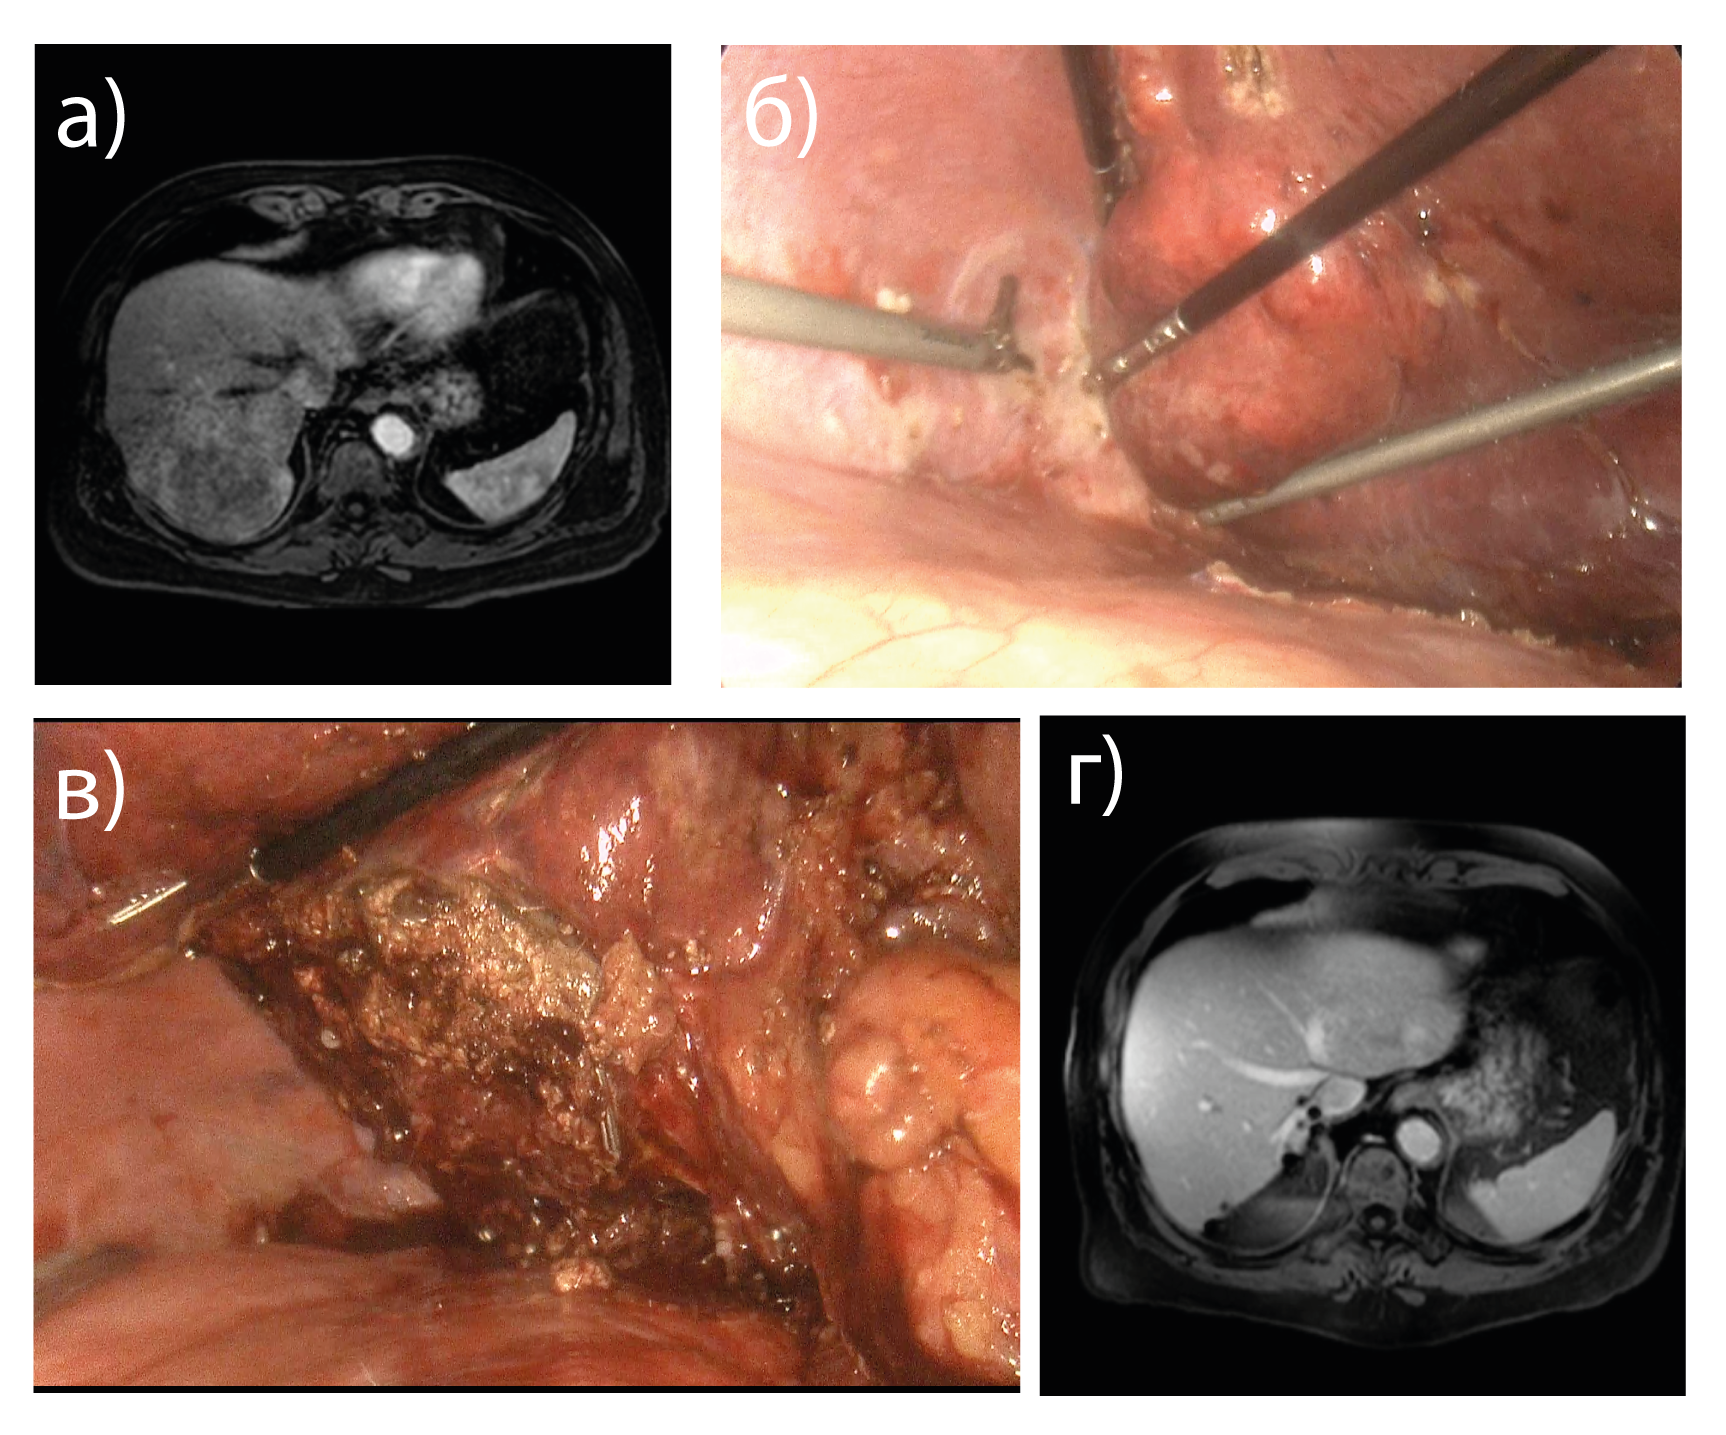
\includegraphics[width=0.9\textwidth]{Illustrations/Chapter_01/Complex_localisation_Sg7.png}
\label{fig:Complex_localisation_Sg7}

\medskip
\small
а) передопераційне \acrshort{mri} \acrshort{hcc}. Пухлина розміром 5 см. розташована в Sg 7,  б) діафрагмальна поверхня Sg 7 печінки з пухлиною, в) резекційна поверхня, г) післяопераційне \acrshort{mri} через 3 місяці після операції.

\end{figure}


\begin{figure}[h]
\caption{Лапароскопічна резекція Sg 8 з приводу ехінококозу у виконанні авторів}

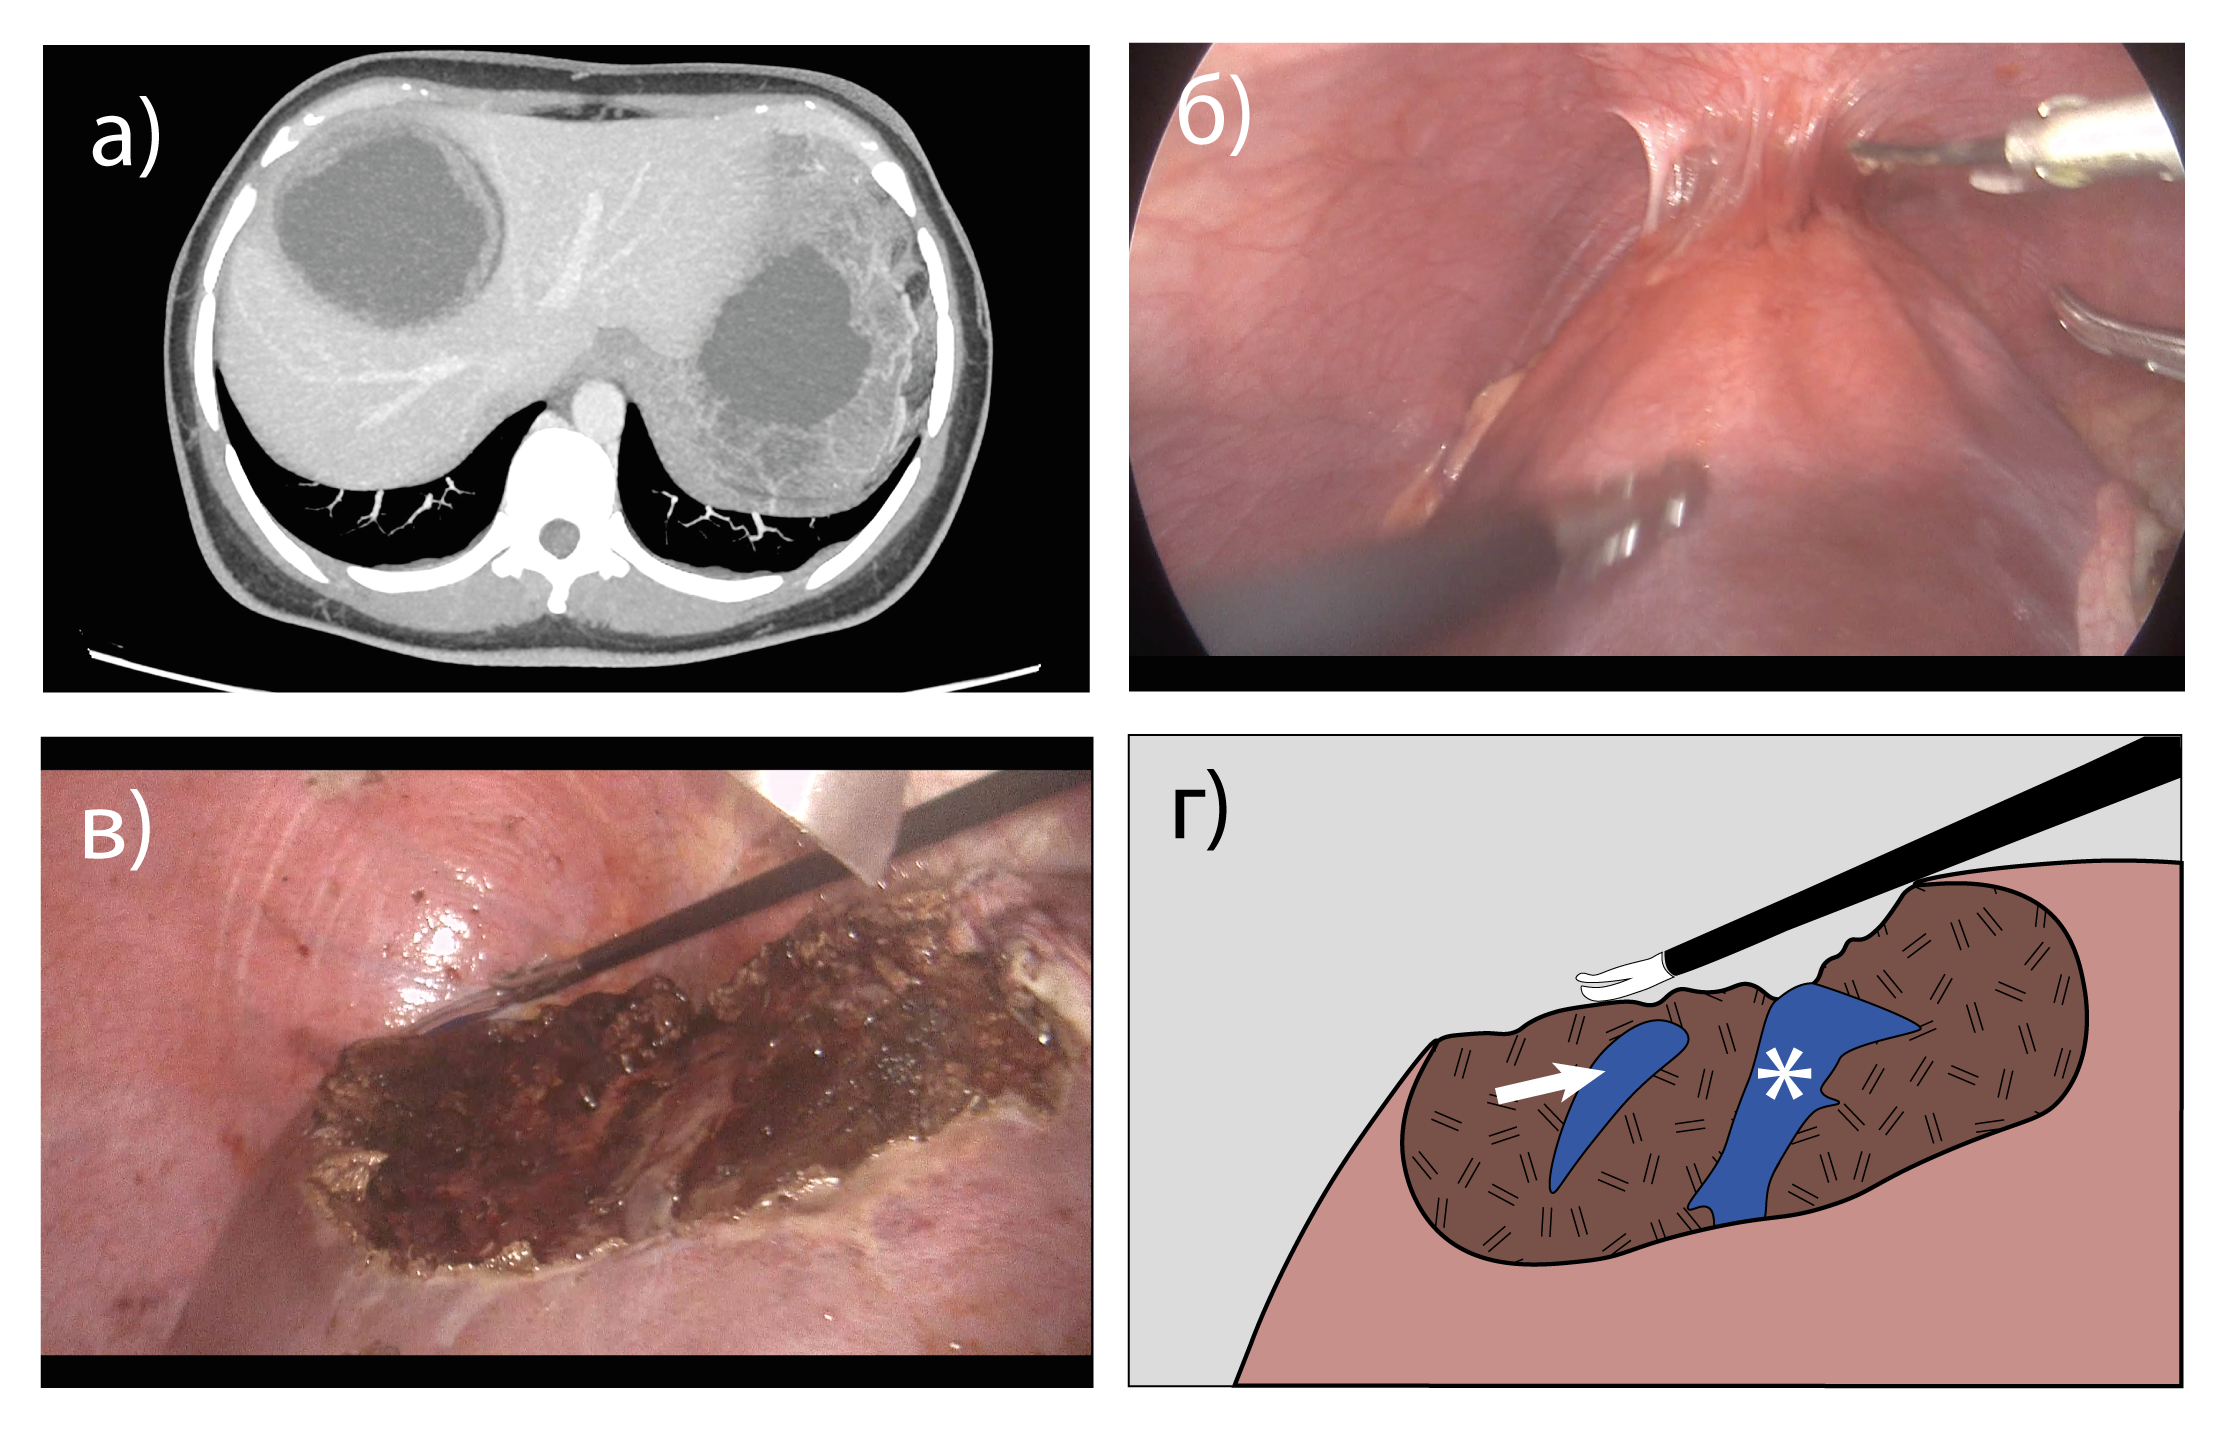
\includegraphics[width=0.9\textwidth]{Illustrations/Chapter_01/Complex_localisation_Sg8.png}
\label{fig:Complex_localisation_Sg8}

\medskip
\small
а) \acrshort{ct} ехінококової кисти, яка прилягає до  серединної печінкової вени, б) діафрагмальна поверхня Sg 8 печінки з кистою, в) резекційна поверхня, г) устя серединної та лівої печінкових вен (відмічено зірочкою) та приток правої печінкової вени (помічено стрілкою) в площині резекції.

\end{figure}





Складність каудальної лобектомії обумовлена тим, що перший сегмент розташований в позаду печінки і безпосередньо межує з \acrshort{ivc}, що робить його пряму візуалізацію неможливою та суттєво ускладнює хірургічний доступ. Окрім того каудальна доля має власні окремі печінкові вени, які дренуються в запечінковий сегмент \acrshort{ivc}, що підвищує ризик кровотечі під час його мобілізації і робить лапароскопічну каудальну лобектомію (\acrshort{lce}) складним втручанням. 
    
В літературі є обмежені згадки про досвід виконання \acrshort{lce} переважно у вигляді кейс-репортів та невеликих серій \cite{Machado2018, Cheung2016, Koh2017, Jin2018}. Найбільшою небезпекою, пов'язаною \acrshort{lce} вважають ризик розвитку масивної неконтрольованої кровотечі з передньої стінки \acrshort{ivc} або задньої стінки серединної печінкової вени (\acrshort{mhv}), при цьому загальна морбідність складає лише 6,6\% \cite{Araki2018}. Альтернативою до лапароскопічного підходу для виконання каудальної лобектомії може стати використання роботичних систем, які полегшують маніпуляції в обмеженому просторі \cite{Marino2018a}.

\subsection[Комплексні резекції]{Комплексні резекції у поєднанні з резекцією судин чи жовчних протоків, розширеною лімфодиссекцією}

У  пацієнтів з поширеними формами метастазів колоректального раку в печінку (\acrshort{crlm}), \acrshort{hcc} чи \acrshort{phcc}  може спостерігатись інвазія в магістральні структури печінки - ворітну вену, печінкові вени або жовчні протоки. Такі пацієнти потребують хірургічного лікування у вигляді резекції печінки в комбінації із судинною або біліарною резекцією. В більшості випадків необхідність комплексної резекції є показом до відкритого втручання, проте деякими авторами описана можливість виконання таких втручань в лапароскопічному варіанті. \cite{Kobayashi2015, Tardu2016, Procopio2020, Matsukuma2020}.

\subsubsection{Резекції судин}

В літературі наявні згадки про невелику кількість випадків резекцій магістральних судин виконаних під час проведення лапароскопічної резекції печінки - 3 кейс-репорти та одне дослідження серії з 6 хворих. 

Так Nomi T. та співавт. повідомляють про успішний випадок крайової резекції \acrshort{ivc} під час проведення \acrshort{lrhe} переднім доступом у 58-річного пацієнта з приводу \acrshort{crlm} \cite{Nomi2015a}. Пізніше Vega E. та співавт. виконали \acrshort{lce} з частковою резекцією \acrshort{ivc} 54-річному пацієнту, що страждав \acrshort{hcc} на фоні цирозу \cite{Vega2020}. 

Lopez-Ben та співавтори показали двохетапний лапароскопічний підхід при видаленні білобарних \acrshort{crlm} 66-річному пацієнту (Рис. \ref{fig:Vascular_resection}) . Першим етапом була виконана лапароскопічна правобічна задня секцієектомія (\acrshort{lrps}) з резекцією та реконструкцією шляхом формування судинного анастомозу правої печінкової вени (\acrshort{rhv}). Під час другого етапу була виконана \acrshort{llhe}. Автори повідомляють про хороший онкологічний ефект операції та відсутність рецидивів під час огляду через 2 роки після втручання \cite{Lopez-Ben2020}.

\begin{figure}[!ht]
\caption{Лапароскопічна правобічна секцієектомія як перший етап двоетапної резекції з приводу \acrshort{crlm} у виконанні Lopez-Ben \cite{Lopez-Ben2020}}

\includegraphics[width=0.95\textwidth]{Illustrations/Chapter_01/Vascular_resection.png}
\label{fig:Vascular_resection}

\medskip
\small
а) \acrshort{ct} \acrshort{crlm}, який прилягає до правої печінкової вени, б) лінія демаркації після перетискання глісону правої задньої секції печінки, в,г) інвазія метастазу в праву печінкову вену (пухлина помічена зірочкою, вена відмічена на схемі синім кольором), ґ, д) резекція стовбура правої печінкової вени, е) реконструкція правої печінкової вени анастомозом кінець в кінець, є) фінальний вигляд вени після накладання анастомозу (лінія анастомозу відмічена пунктиром)

\end{figure}
	
Єдине дослідження серії випадків судинних резекцій під час проведення \acrshort{llr} належить Morise Z. та співавторам \cite{Morise2015a}. Автори заявляють про досвід 98 \acrshort{llr} з приводу \acrshort{hcc} на фоні цирозу, 6 з яких було виконано резекцію стовбура однієї з магістральних печінкових вен за допомогою лінійного степлера.

Не дивлячись на достатньо поширене застосування резекції та реконструкції стовбура ворітної вени під час виконання лапароскопічної панкреатодуоденальної резекції \cite{Kendrick2011, Garbarino2018, Wei2019} нами не було знайдено джерел, що описують застосування портопластики під час проведення \acrshort{llr}, що скоріше за все пов'язано із її технічною складністю та обмеженістю показів. 

\subsubsection{Біліарні реконструкції}

В лапароскопічному варіанті, як самостійне втручання гепатикоєюностомія широко використовується при кистах та стриктурах холедоха, як паліативне втручання, а також як частина панкреатодуоденальної резекції при пухлинах голівки підшлункової залози. Резекція позапечінкових жовчних шляхів є обов'язковим етапом радикальних резекцій печінки з приводу \acrshort{phcc} а також може бути застосована при пухлинній інвазії іншими пухлинами. Згідно доступних даних \acrshort{llr} з приводу  \acrshort{phcc} все ще є новітньою процедурою на стадії вивчення, тому досвід виконання таких операцій обмежений кейс-репортами \cite{Lin2014, Machado2014} або невеликими серіями \cite{Ratti2020}. Таким чином в експертних центрах гепатикоєюностомія є технічно доступним етапом при виконанні \acrshort{llr}, а впровадження роботичної хірургії дає надію на її більш широке застосування \cite{Machado2019, Giulianotti2010}

\subsubsection{Розширена лімфаденектомія}

Лімфодиссекція є стандартизованим етапом багатьох лапароскопічних операцій з приводу онкопатології, зокрема в мініінвазивній гінекології та хірургії шлунково-кишкового тракту \cite{Eshuis2018, Jung2019}. В резекційній хірургії печінки лімфодиссекція показана при наявності локального позапечінкового ураження лімфовузлів наприклад при \acrshort{crlm}. Не дивлячись на те, що  онкологічна ефективність привентивної лімфаденектомії при \acrshort{llr} з приводу \acrshort{ihcc} остаточно не доведена \cite{Weber2015, Zhou2019a}, багато хірургів рекомендують її рутинне виконання з метою адекватного стадіювання пухлини та визначення прогнозу \cite{Waisberg2018, Ratti2020a}.

Більшість данних про лімфаденектомію як етап \acrshort{llr} представлені у вигляді кейс-репортів та серій випадків. Їх узагальнення  наведено Levi Sandri G.B. та співавторами в оглядовій статті, на основі чого автори роблять висновок про безпечність та доступність лапароскопічного підходу \cite{Colasanti2017}. 

Також є результати моноцентрового псевдорандомізованого дослідження в якому Ratti F. зі співавторами порівнюють 20 пацієнтів, що перенесли \acrshort{llr} з приводу \acrshort{ihcc} із 60 аналогічними відкритими операціями. За отриманими результатами \acrshort{llr}, серед яких 85\% великих резекцій, були не гіршими від відкритих втручаннь за показниками морбідності та безрецидивної виживаності, а також були асоційовані із меншою крововтратою та більшою кількістю видалених лімфовузлів \cite{Ratti2016a}. 

\subsection{Технологія ALPPS} 

В перше технологія Associating Liver Partition and Portal vein Ligation for Staged hepatectomy(\acrshort{alpps}) була запропонована в 2011  Lang H.  \cite{Baumgart2011} в якості альтернативи звичайній двоетапній резекції печінки з лігуванням ворітної вени. Суть нововведення полягала в тому, що на першому етапі проводять санацію планованого печінкового залишку, лігування ворітного притоку  частини печінки, що видаляють та транссекція паренхіми. При цьому за рахунок потужного викиду прозапальних факторів протягом 7-14 днів відбувається швидкий приріст об'єму планованого печінкового залишку, після чого виконують другий етап, під час якого видаляють депорталізовану на першому етапі частину печінки. 

Методика привернула увагу та отримала багатьох прихильників серед гепатобіліарних хірургів, як метод, що дозволяє значно розширити межі резектабельності у пацієнтів з обширним пухлинним ураженням. Критики цієї методики зазначають, що вона має високу частоту післяопераційних ускладненнь та ризики прогрессії пухлини між першим та другим етапами. 

Для подолання цих недоліків Brustia R. та співавторами було запропоновано виконувати втручання в лапароскопічному варіанті \cite{Brustia2013}. Наразі загальна кількість таких операцій не велика, що може бути пов'язано з тим, що відкрита  \acrshort{alpps} є відносно новим та методом, який досі знаходиться на етапі дослідження \cite{Melandro2019}.

Так, Michal K. та співавтори \cite{Michal2020} за результатами метааналізу 23 джерел порівняли 46 мініінвазивних та 1088 відкритих \acrshort{alpps}, та дійшли до висновку, що лапароскопічні та роботичні втручання дозволяють знизити частоту ускладненнь порівняно з відкритими втручаннями та отримати більший ступінь гіпертрофії порівняно з емболізацією ворітної вени. 

\subsection{Лапароскопічна донорська резекція печінки} 

Трансплантація печінки від живого донора стала радикальним методом лікування дифузних захворюваннь та деяких пухлин печінки в умовах відсутності або обмеженої кількості трупних донорів. На відміну від резекцій з приводу новоутвореннь, під час виконання донорської резекції печінки перед хірургом стоять два завдання -  забезпечення безпеки та збереження здоров'я донора та забір реплантабельного та функціонального трансплантату з достатньою довжиною та придатним для пластики краєм ворітної та печінкових вен, печінкової артерії та жовчних протоків. 

Для зменшення ризику ускладненнь та раннього повернення працездатності донору в 2002 р. Cherqui D. та співавторами було запропоновано виконання донорського забору лівої латеральної секції в лапароскопічному варіанті при трансплантації дітям \cite{Cherqui2002a}. Пізніше техніка операції була адаптована та імплементована деякими центрами. Так наприклад Kim K-H. та свпіватори повідомляють про переваги лапароскопічного донорського забору лівої латеральної секції у вигляді зменшення терміну госпіталізації та пришвидшення реабілітації донора за результатами порівняння 11 таких втручаннь із 11 відкритими донорськими резекціями \cite{Kim2011}. 

Технічно більш складна донорська правобічна гемігепатектомія певний час залишалась недоступною для чисто лапароскопічного доступу. Запропоновані \acrshort{hals} та \acrshort{hlr} підходи не набули широкого розповсюдження \cite{Koffron2006, Thenappan2011, Lin2013}. Лише в 2013 р. Soubrane O. та співавторами була показана можливість донорського забору трансплантату правої долі печінки в чисто лапаропскопічному доступі \cite{Soubrane2013}. 

На теперішній момент лапароскопічний донорська гепатектомія активно застосовується більшістю великих спеціалізованих трансплантаційних центрів. Доступні результати псевдорандомізованих порівняльних дослідженнь, які демонструють переваги лапароскопічних донорських заборів над відкритими \cite{Broering2018, Park2019a}. Також показано безпеку лапароскопічного забору для реципієтнів \cite{Kwon2018a}. Йде дискуссія про стандартизацію та повсюдне впровадження методу \cite{Au2018, Samstein2018}

Таким чином за свою майже 30-річну історію \acrshort{llr} вийшла далеко за межі крайових та атипових резекцій антеролатеральних сегментів та впевнено конкурує з відкритими втручаннями у всіх галузях гепатобіліарної хірургії. 